\documentclass{article}

\usepackage[english]{babel}
\usepackage[letterpaper,top=2cm,bottom=2cm,left=3cm,right=3cm,marginparwidth=1.75cm]{geometry}
\usepackage{amsmath}
\usepackage{graphicx}
\usepackage{float}
\usepackage{listings}
\usepackage{xcolor}
\usepackage{url}
\usepackage[colorlinks=true, allcolors=blue]{hyperref}

\lstdefinestyle{docker}{
    backgroundcolor=\color{gray!5},
    basicstyle=\ttfamily\small,
    frame=single,
    rulecolor=\color{black!30},
    breaklines=true,
    postbreak=\mbox{\textcolor{red}{$\hookrightarrow$}\space},
    keywordstyle=\color{blue}\bfseries,
    commentstyle=\color{gray}\itshape,
    numbers=left,
    numberstyle=\tiny\color{gray},
    stepnumber=1,
    numbersep=8pt,
    captionpos=b
}

\lstdefinestyle{pythoncode}{
    backgroundcolor=\color{gray!5},
    basicstyle=\ttfamily\small,
    frame=single,
    rulecolor=\color{black!30},
    breaklines=true,
    postbreak=\mbox{\textcolor{red}{$\hookrightarrow$}\space},
    keywordstyle=\color{blue}\bfseries,
    stringstyle=\color{orange!80!black},
    commentstyle=\color{gray}\itshape,
    numbers=left,
    numberstyle=\tiny\color{gray},
    stepnumber=1,
    numbersep=8pt,
    captionpos=b
}

\lstdefinelanguage{yaml}{
  keywords={true,false,null,y,n},
  keywordstyle=\color{blue}\bfseries,
  basicstyle=\ttfamily\small,
  sensitive=false,
  comment=[l]{\#},
  morecomment=[s]{/*}{*/},
  commentstyle=\color{gray}\itshape,
  stringstyle=\color{orange!80!black},
  morestring=[b]',
  morestring=[b]"
}

\author{George Lipceanu (20103125)}
\date{October 14., 2025}

\begin{document}

\begin{titlepage}
    \centering
    
    \vspace*{2cm}
    
    {\Huge \textbf{Sustainable Kubernetes Extension Stack} \par}
    \vspace{1cm}
    {\Large \textit{Final Year Project}\par}
    \vspace{1.5cm}
    
    {\Large George Lipceanu (20103125)\par}
    \vspace{0.5cm}
    
    {\large October 14, 2025\par}
    
    \vspace{3cm}
    
    \tableofcontents
    
    \vfill
\end{titlepage}


\newpage         

\section{Introduction}
This project delivers an opinionated, end-to-end sustainability extension stack for Kubernetes. It integrates
\emph{Custom Resource Definitions (CRDs)}, \emph{reconciling controllers}, and a \emph{carbon-aware scheduler plugin}
into a cohesive system that makes energy and carbon first-class signals in cluster operations. A companion CLI
 automates installation, upgrades, and cluster validation, while an observability layer
(Prometheus + Grafana) exposes real-time power, energy, and emission metrics.

\paragraph{Problem Statement}
Kubernetes optimises for resource fit, availability, and fairness, 
but lacks native constructs to reason about energy or carbon. Operators 
cannot declaratively express sustainability intent, like favouring lower-intensity nodes. 
or audit the energy and emissions impact of workloads without ad-hoc tooling.

\paragraph{Vision}
Make sustainability declarative, actionable, and measurable for Kubernetes workloads by:
(i) modelling carbon and energy as API resources; (ii) reconciling cluster state toward sustainability intent; and
(iii) feeding those signals into scheduling and reporting decisions.

\paragraph{Scope}
The stack provides:
\begin{itemize}
  \item \textbf{APIs}: CRDs for carbon intensity, workload policies, and emission reports.
  \item \textbf{Controllers}: Operators that fetch carbon data, apply workload policies, and provide data on energy saved, emissions, etc..
  \item \textbf{Scheduler Plugin}: Scheduler that combines standard utilisation bin-packing with carbon-aware scoring.
  \item \textbf{External Components}: Kepler for node-level power estimation, Prometheus for metric collection, Grafana for dashboards.
  \item \textbf{Tooling}: CLI binaries to install, configure, and inspect the stack and clusters data.
\end{itemize}

\paragraph{Design Principles}
\begin{enumerate}
  \item \textbf{Upstream compatibility}: built on the Kubernetes Scheduling Framework and CRD APIs.
  \item \textbf{Separation of concerns}: making sure each component in the system does one thing well.
  \item \textbf{Clear intent}: sustainability is defined through CRDs and labels.
  \item \textbf{Observability by default}: all sustainability data are inspectable via metrics and dashboards.
  \item \textbf{Fault tolerance}: provider failures fall back to last-known-good or neutral scores.
\end{enumerate}

\paragraph{Implementation Overview}
The system is implemented in Go using Kubebuilder for operator scaffolding. The custom scheduler plugin ingests
(i) node utilisation, (ii) carbon intensity signals from CRDs or cached ConfigMaps, and (iii) workload policies
to compute a composite score per node. Prometheus scrapes Kepler and controller metrics, with Grafana visualising energy,
emission, and placement data. The CLI automates installation, upgrades, and basic diagnostics.

\subsection{Motivation}

Cloud workloads are increasingly energy-intensive, yet most platforms obscure their carbon impact. Teams cannot easily
answer:
\begin{enumerate}
  \item Where did this workload run?
  \item How much energy did it consume?
  \item Could this energy use have been reduced?
\end{enumerate} 

With AI/ML and data-processing clusters growing rapidly, a practical way to measure, optimise, and
report sustainability at the orchestration layer is timely. This project addresses that gap through three core capabilities:
\begin{enumerate}
  \item \textbf{Measurement}: Kepler-based power and energy estimation linked to workloads over time.
  \item \textbf{Optimisation}: a scheduler that prefers lower-intensity, highly-utilised nodes (bin-pack + carbon scoring).
  \item \textbf{Reporting}: CRD-driven policies and auditable emission reports for teams and compliance, alongside observability in Grafana dashboards.
\end{enumerate}

\subsection{Review of Related Work}

\paragraph{Energy/Carbon-Aware Scheduling}
Existing research and community prototypes extend scheduling logic with sustainability signals, often combining resource
fit with energy or carbon metrics. This work follows that approach but maintains upstream compatibility through the
Kubernetes Scheduling Framework, avoiding invasive patches to the core scheduler.

\paragraph{Telemetry and Power Modelling}
Kepler estimates node and container energy using eBPF (extended Berkeley Packet Filter) and hardware counters, exporting metrics consumable by Prometheus.
For real-time scheduling, a linear node-level power model is used as shown below:
\[
P = P_{\text{idle}} + U_{\text{cpu}}\,(P_{\text{max}} - P_{\text{idle}})
\]

\paragraph{Policy and Governance}
This project expresses sustainability constraints declaratively 
through CRDs such as \texttt{WorkloadPolicy}, allowing schedulers and 
controllers to consume consistent signals without bespoke integrations 
for each workload.

\paragraph{Carbon Data Providers}
Operational systems commonly query regional carbon intensity from external providers. This stack encapsulates provider
interactions in the \texttt{CarbonInfoController}, which normalises units, updates CRD status, and writes a cached
ConfigMap. The scheduler reads from this cache, ensuring deterministic behaviour even under provider outages.

\paragraph{Positioning}
This work is fully Kubernetes-native. Sustainability intent is declared via
CRDs, enforced by reconcilers, enacted at scheduling time, and validated post-hoc through emission reports and metrics.
The emphasis is on practicality—achieving measurable sustainability impact with minimal operational overhead.

\section{System Architecture and Design}

\subsection{CRDs}

Custom Resource Definitions capture sustainability signals and preferences as Kubernetes-native APIs.
They include OpenAPI validation, defaults, and standard status conditions and are built using Kubebuilder. 
Controllers reconcile these resources and project their outputs to the
scheduler and observability stack.

\paragraph{Summary of CRDs}
\begin{itemize}
  \item \textbf{CarbonInfo}: normalises grid carbon intensity per region or node group.
  \item \textbf{WorkloadPolicy}: defines carbon-aware scheduling preferences and thresholds for labelled workloads.
  \item \textbf{EmissionReport}: aggregates energy and carbon emissions over a reporting window.
\end{itemize}

\paragraph{CarbonInfo}
\textit{Purpose}: represent regional or node-group carbon intensity as a live signal.

\noindent\textbf{Spec (key fields)}
\begin{itemize}
  \item \texttt{provider}: data source (mock, ElectricityMap, or static).
  \item \texttt{region}: provider-specific key.
  \item \texttt{pollSeconds}: refresh cadence for live data.
  \item \texttt{staticIntensity}: fallback or fixed gCO\textsubscript{2}/kWh for static mode.
\end{itemize}

\noindent\textbf{Status (key fields)}
\begin{itemize}
  \item \texttt{currentIntensity}: latest gCO\textsubscript{2}/kWh value.
  \item \texttt{lastUpdated}: timestamp of last successful update.
  \item \texttt{conditions}: readiness and error states.
\end{itemize}

\paragraph{WorkloadPolicy}
\textit{Purpose}: declaratively express carbon-aware scheduling preferences for matching workloads.

\noindent\textbf{Spec}
\begin{itemize}
  \item \texttt{target}: label and namespace selectors defining workloads in scope.
  \item \texttt{maxCarbonIntensity}: upper bound (gCO\textsubscript{2}/kWh) for eligible nodes.
  \item \texttt{schedulerHints}: optional key-value hints such as 
        \texttt{utilisationWeight: 0.7}, \texttt{carbonWeight: 0.3}.
  \item \texttt{enforcement}: \texttt{soft} (prefer) or \texttt{hard} (require).
\end{itemize}

\noindent\textbf{Status}
\begin{itemize}
  \item \texttt{enforced}: whether hints are applied to all matching workloads.
  \item \texttt{matchedWorkloads}: count of affected workloads.
  \item \texttt{conditions}: reconciliation results.
\end{itemize}

\paragraph{EmissionReport}
\textit{Purpose}: summarise cluster-wide or workload-level energy and emission metrics into auditable reports.

\noindent\textbf{Spec}
\begin{itemize}
  \item \texttt{scope}: aggregation level (namespace, workload, or node).
  \item \texttt{from}, \texttt{to}: timestamps defining the reporting window.
\end{itemize}

\noindent\textbf{Status}
\begin{itemize}
  \item \texttt{totals}: overall energy (kWh) and emissions (gCO\textsubscript{2}) for the report period.
  \item \texttt{breakdown}: per-namespace/workload/node details.
  \item \texttt{conditions}: \texttt{Finished} or \texttt{DataPartial} with current info.
\end{itemize}

\paragraph{Validation and Security}
CRDs include OpenAPI validation to enforce schema correctness.
Controllers run with minimal RBAC privileges and operate
namespace-scoped for multi-tenant isolation.

\subsection{Controller Logic}

Controllers follow the operator reconciliation pattern to align cluster state with declarative sustainability intent.
Each controller observes its CRD, updates \texttt{status}, and publishes derived data to the scheduler or metrics system.

\paragraph{CarbonInfoController}
\begin{itemize}
  \item \textbf{Watches}: \texttt{CarbonInfo} resources.
  \item \textbf{External I/O}: queries carbon intensity from configured providers.
  \item \textbf{Actions}: updates CRD status, maintains \texttt{ready}/\texttt{unavailable} conditions, and writes a
        cached ConfigMap mapping nodes or regions to intensity values for the scheduler plugin.
\end{itemize}

\paragraph{WorkloadPolicyController}
\begin{itemize}
  \item \textbf{Watches}: \texttt{WorkloadPolicy} and corresponding \texttt{Jobs}/\texttt{Pods}/\texttt{Deployments}.
  \item \textbf{Actions}: validates policy and injects hints via annotations and labels,
        sets \texttt{spec.schedulerName: carbon-scheduler} when required,
        updates \texttt{status.enforced}.
  \item \textbf{Scheduler Integration}: the scheduler plugin reads these hints during the scoring process to
        adjust weighting and eligibility.
\end{itemize}

\paragraph{EmissionReportController}
\begin{itemize}
  \item \textbf{Watches}: \texttt{EmissionReport} resources.
  \item \textbf{Inputs}: Prometheus and Kepler metrics (CPU usage, power), \texttt{CarbonInfo} intensities.
  \item \textbf{Actions}: queries metrics over the report window, calculates energy consumption using the linear power model,
        multiplies by carbon intensity to estimate emissions, and writes totals and breakdowns to \texttt{status}.
\end{itemize}

\paragraph{Data Flow Summary}
\begin{enumerate}
  \item \textbf{CarbonInfoController} fetches carbon intensity and updates CRD status and cache.
  \item \textbf{WorkloadPolicyController} injects scheduling thresholds and pre-reqs into targeted workloads.
  \item \textbf{Scheduler Plugin} reads utilisation, policies, and cached carbon data to score nodes and bind pods.
  \item \textbf{EmissionReportController} queries metrics and produces reports of energy and emissions.
\end{enumerate}

\begin{figure}[H]
  \centering
  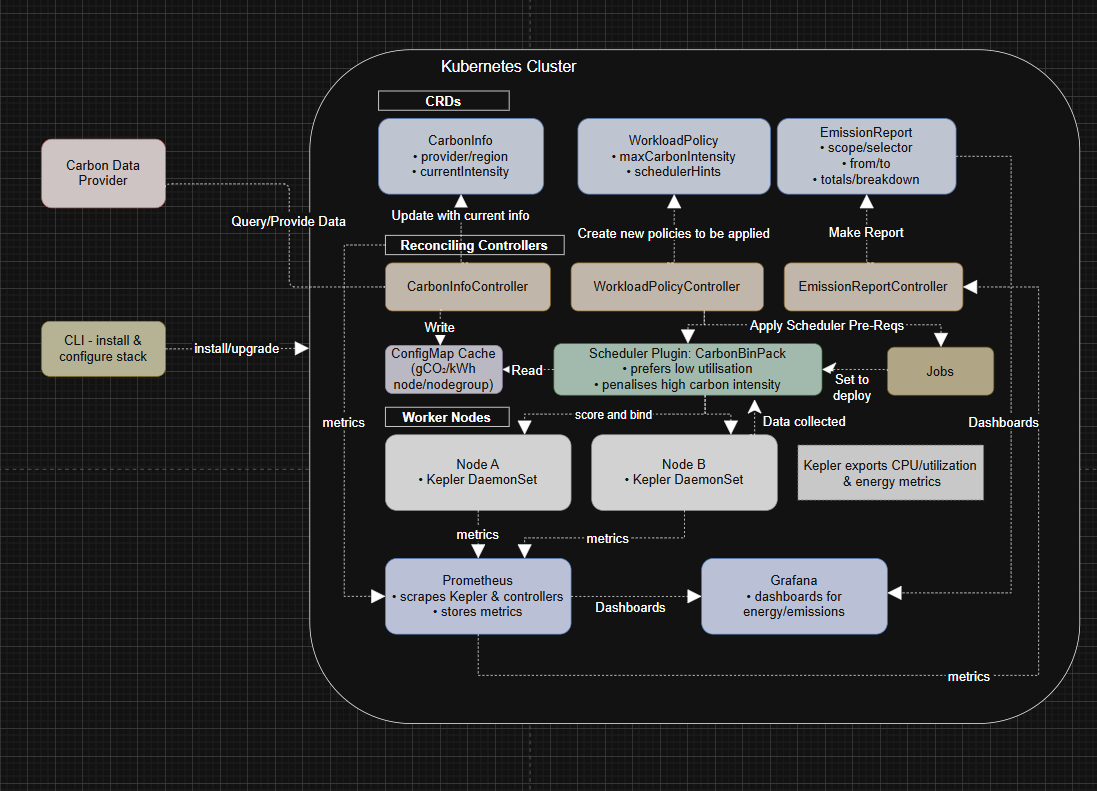
\includegraphics[width=0.95\textwidth]{figures/system_diagram.png}
  \caption{Overall architecture of the Sustainable Kubernetes Extension Stack.}
  \label{fig:system_diagram}
\end{figure}

\paragraph{Operational Notes}
\begin{itemize}
  \item Controllers are idempotent and reconcile periodically or on CRD change events.
  \item The controllers pre-compute data required for constant-time scoring for scheduler, minimising scheduling time.
\end{itemize}


\section{Scheduler Design and Implementation}

The Kubernetes scheduler is responsible for assigning unscheduled Pods to available Nodes.  
When a new Pod is created without a \texttt{spec.nodeName}, the scheduler sees it, evaluates all available Nodes, selects the best Node according to cluster policy, and writes the Node name back to the Pod object.
The scheduler continuously watches for pending Pods and reacts to changes in cluster state and its primary goal is to ensure efficient resource utilisation and fairness across workloads.\cite{k8s-docs}

\subsection{Implementation Structure}

The scheduler source code can be found in the \texttt{pkg/scheduler/} directory of the Kubernetes repository. The main interfaces are:

\begin{itemize}
  \item \textbf{Filter} --- decide whether a Node is feasible.
  \item \textbf{Score} --- rank feasible Nodes with an integer 0--100.
  \item \textbf{PreBind / Bind / PostBind} --- finalise scheduling.
\end{itemize}

Each phase is implemented through the \textit{Scheduling Framework}, which provides plugin interfaces located in \texttt{pkg/scheduler/framework/}. This modularity allows custom policies to be added without modifying core logic \cite{scheduling-framework-proposal}.

\subsection{Filtering Phase}

In the filtering phase, the scheduler evaluates each Node against a set of constraints implemented by \textbf{Filter plugins}.  
Typical filters include:

\begin{itemize}
  \item \textbf{NodeResourcesFit:} Ensures that the Node has sufficient CPU and memory.
  \item \textbf{TaintToleration:} Verifies that the Pod can tolerate Node taints.
\end{itemize}

Nodes that pass all filters are added to the list of feasible Nodes.

\subsection{Scoring Phase and Scheduling Formula}

Once feasible Nodes are determined, each is scored by multiple \textbf{Score plugins}.  
These plugins assign integer scores in the range $[0, 100]$.  
The final scheduling decision is based on a weighted combination of all plugin scores.

\subsection{Configuration and Extensibility}

The scheduler is configured using a \texttt{KubeSchedulerConfiguration} object.  
An example configuration is shown below:

\begin{verbatim}
apiVersion: kubescheduler.config.k8s.io/v1beta3
kind: KubeSchedulerConfiguration
profiles:
- schedulerName: default-scheduler
  plugins:
    score:
      enabled:
      - name: NodeResourcesFit
  pluginConfig:
  - name: NodeResourcesFit
    args:
      scoringStrategy:
        type: MostAllocated
\end{verbatim}

Pods can opt into a specific scheduler profile by setting:

\begin{verbatim}
spec:
  schedulerName: default-scheduler
\end{verbatim}

This configuration-based design allows different workloads to use different scheduling policies within the same cluster.

\subsection{Modified Scheduler Design for Sustainability}

While the vanilla Kubernetes scheduler focuses on resource allocation and fairness, it does not consider the environmental impact of workload placement.  
This project extends this mechanism by introducing carbon-aware scheduling, enabling Pods to be assigned to Nodes that minimise energy consumption and emissions.  
This is achieved through the addition of a new scoring plugin, implemented using the Kubernetes Scheduling Framework API.  
The plugin integrates data from sustainability metrics and resource utilisation to make more environmentally efficient scheduling decisions.

\subsubsection{Design Objectives}

The primary goals of the modified scheduler are:
\begin{itemize}
  \item Reduce energy usage by consolidating workloads onto fewer, more efficiently utilised Nodes.
  \item Maintain compatibility with upstream Kubernetes.
\end{itemize}

\subsubsection{Implementation Details}

The plugin is implemented under 
\texttt{pkg/scheduler/carbonfit/plugin.go} and registered in \texttt{cmd/kube-scheduler/main.go}. The
Scoring logic for the sample is shown below (based on other plug-ins):

\begin{verbatim}
func (p *Plugin) Score(ctx context.Context, state *framework.CycleState,
  pod *v1.Pod, nodeName string) (int64, *framework.Status) {

  ni, _ := p.handle.SnapshotSharedLister().NodeInfos().Get(nodeName)
  used := ni.Requested.MilliCPU
  alloc := ni.Allocatable.MilliCPU
  utilisation := float64(used) / float64(alloc)

  // Base score favors high utilisation (bin-packing)
  score := int64(utilisation * 100)

  // Incorporate carbon intensity from CRD
  carbonIntensity := 250.0 // gCO2/kWh (static example)
  penalty := int64((1 - utilisation) * carbonIntensity / 10)

  final := score - penalty
  if final < 0 { final = 0 }

  return final, framework.NewStatus(framework.Success, "")
}
\end{verbatim}

This logic favors Nodes that are well utilised and penalises those with higher carbon intensity, balancing performance with environmental cost.

\subsubsection{Configuration Example}

\begin{verbatim}
apiVersion: kubescheduler.config.k8s.io/v1beta3
kind: KubeSchedulerConfiguration
profiles:
- schedulerName: susk8s-scheduler
  plugins:
    score:
      enabled:
      - name: CarbonBinPack
      - name: NodeResourcesFit
  pluginConfig:
  - name: CarbonBinPack
    args:
      UtilisationWeight: 0.7
      CarbonWeight: 0.3
\end{verbatim}

\subsubsection{Emission Estimation}
The total energy consumption of a Node over time is modeled as a function of its CPU utilisation.  
Each Node has a characteristic power profile defined by its \textbf{idle power} ($P_{idle}$) and \textbf{maximum power} ($P_{max}$).  
The scheduler assumes that power consumption grows linearly with CPU usage, following the linear CPU power model established by Lin et al. (2021), introduced in Section 2.2 of \cite{Lin2021HCPM}.  
This model provides a balance between accuracy and computational simplicity, making it well suited for real-time scheduling decisions within a Kubernetes control loop. 
This makes the model sufficiently accurate for cluster-level energy and carbon estimations while remaining architecture-agnostic and lightweight to compute.

The instantaneous power draw $E_n$ (in watts) for a Node $n$ is thus estimated as:

\[
E_n = P_{idle} + U_{cpu} \times (P_{max} - P_{idle})
\]

where:
\begin{itemize}
  \item $E_n$ is the estimated node power draw in watts.
  \item $P_{idle}$ represents the baseline power consumed when the node is idle.
  \item $P_{max}$ represents the power at full CPU utilisation.
  \item $U_{cpu}$ is the current CPU utilisation ratio, obtained from metrics exported by Kepler (\texttt{container\_cpu\_usage\_seconds\_total}).\cite{kepler}
\end{itemize}

This power is then integrated over the task's duration, resulting in energy in joules or kilowatt-hours (kWh):

\[
E_{total} = \int_{t_0}^{t_1} E_n(t) \, dt
\]

Once the total energy consumed ($E_{total}$) is known, it can be converted into greenhouse gas emissions using the regional carbon intensity, $I_{carbon}$, measured in grams of CO$_2$ per kilowatt-hour (gCO$_2$/kWh).  
The emissions are calculated as:

\[
CO_{2total} = E_{total} \times I_{carbon}
\]

where:
\begin{itemize}
  \item $E_{total}$ is the total energy consumed (kWh).
  \item $I_{carbon}$ is obtained from an external provider.
\end{itemize}


\subsection{Impact and Discussion}

This modification introduces sustainability as a first-class concern in Kubernetes scheduling.  
It reduces unnecessary energy usage and enables emission tracking.
It also maintains full compatibility with upstream Kubernetes, demonstrating that sustainability 
can be achieved through simple plugin extensions and also allowing for 
compatibile this same cluster deployment across multiple environments.

\section{Implementation of Supporting Components}

\subsection{Kepler}

Kepler (Kubernetes Efficient Power Level Exporter) is a lightweight component that
estimates energy consumption and power draw at the container 
and node levels. It is deployed as a \texttt{DaemonSet} across all worker
nodes and uses kernel-level counters and hardware performance counters
to determine CPU power.

In this project, Kepler serves two key roles:
\begin{enumerate}
  \item It provides node-level CPU utilisation and power estimation metrics (\texttt{kepler\_container\_joules\_total}, \texttt{kepler\_container\_cpu\_utilization}) that the \texttt{EmissionReportController} consumes.
  \item It supplies instantaneous CPU utilisation values (\texttt{container\_cpu\_usage\_seconds\_total}) to the scheduler via Prometheus queries, enabling energy-aware placement decisions.
\end{enumerate}

Kepler is deployed under the \texttt{kepler} namespace with a \texttt{ClusterRole} 
allowing node and pod metric access. Metrics are exposed at 
\texttt{/metrics} and scraped periodically by Prometheus. 
These values are aggregated and transformed into energy 
(Joules) and emission equivalents by the \texttt{EmissionReportController}, 
enabling correlation between workload identity, energy consumption, and carbon footprint.

\subsection{Prometheus}

\subsection{Grafana}

\subsection{Cobra CLI}

\section{Multi-Cluster Deployments}

\section{Testing and Evaluation}

\section{Summary and Discussion}


\nocite{*}
\bibliographystyle{plainurl}
\bibliography{sample}

\end{document}
